\chapter{Function plots}

In this chapter, we will work towards creating the function plot below.
We will take you from a basic function plot and explain all the
customisations we add to the code step-by-step.

\begin{center}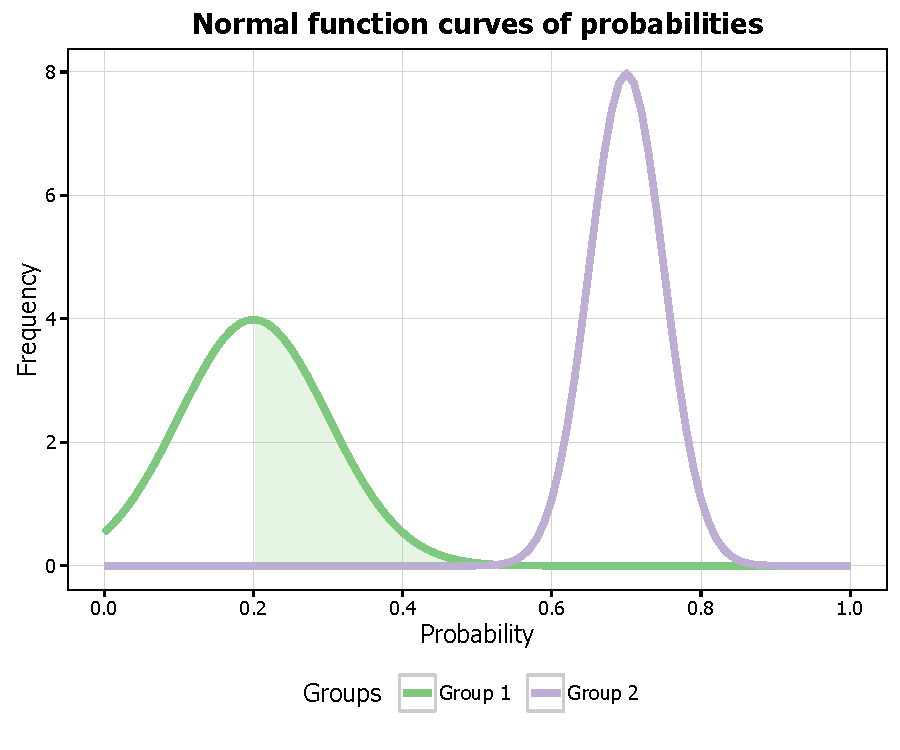
\includegraphics[width=0.6\linewidth]{9_Function_Plots_pdf/function_final-1} \end{center}

The first thing to do is load in the libraries, as below:

\begin{Shaded}
\begin{Highlighting}[]
\KeywordTok{library}\NormalTok{(ggplot2)}
\KeywordTok{library}\NormalTok{(ggthemes)}
\KeywordTok{library}\NormalTok{(grid) }
\KeywordTok{library}\NormalTok{(extrafont)}
\end{Highlighting}
\end{Shaded}

\section{Basic normal curve}\label{basic-normal-curve}

In order to create a normal curve, we create a ggplot base layer that
has an x-axis range from -4 to 4 (or whatever range you want!), and
assign the x-value aesthetic to this range (\texttt{aes(x\ =\ x)}). We
then add the \texttt{stat\_function} option and add \texttt{dnorm} to
the function argument to make it a normal curve.

\begin{Shaded}
\begin{Highlighting}[]
\NormalTok{p9 <-}\StringTok{ }\KeywordTok{ggplot}\NormalTok{(}\KeywordTok{data.frame}\NormalTok{(}\DataTypeTok{x =} \KeywordTok{c}\NormalTok{(-}\DecValTok{4}\NormalTok{, }\DecValTok{4}\NormalTok{)), }\KeywordTok{aes}\NormalTok{(}\DataTypeTok{x =} \NormalTok{x)) +}
\StringTok{  }\KeywordTok{stat_function}\NormalTok{(}\DataTypeTok{fun =} \NormalTok{dnorm)}
\NormalTok{p9}
\end{Highlighting}
\end{Shaded}

\begin{center}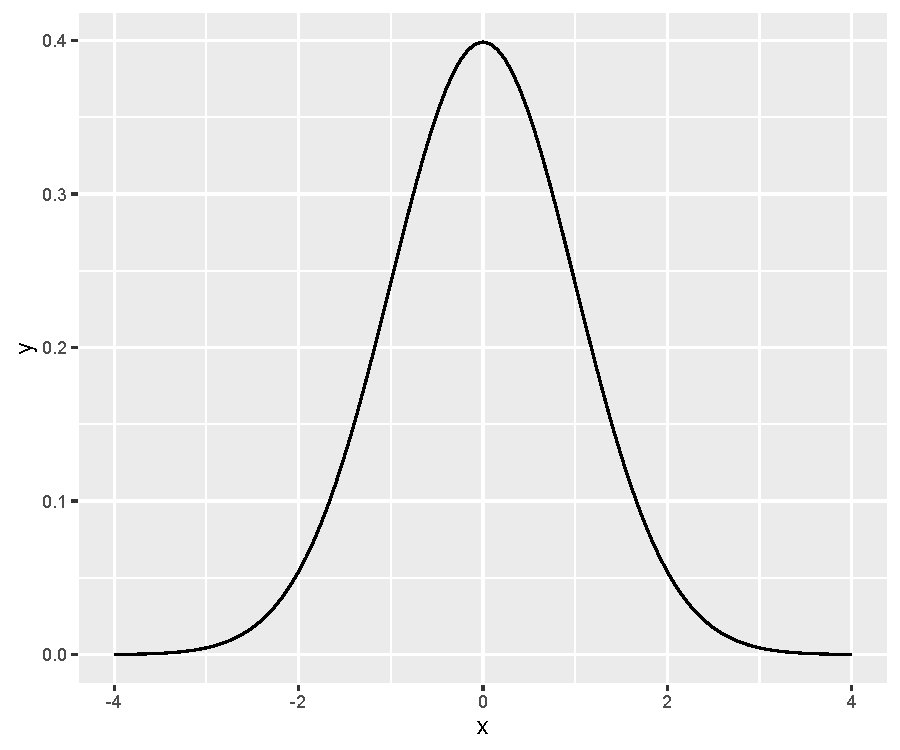
\includegraphics[width=0.6\linewidth]{9_Function_Plots_pdf/function_1-1} \end{center}

\section{Basic t-curve}\label{basic-t-curve}

\texttt{stat\_function} can draw a range of continuous
\href{https://en.wikipedia.org/wiki/Probability_density_function}{probability
density functions}, including t (\texttt{dt}), F (\texttt{df}) and
Chi-square (\texttt{dchisq}) PDFs. Here we will plot a t-distribution.
As the shape of the t-distribution changes depending on the sample size
(indicated by the degrees of freedom, or df), we need to specify our df
value as part of defining our curve.

\begin{Shaded}
\begin{Highlighting}[]
\NormalTok{p9 <-}\StringTok{ }\KeywordTok{ggplot}\NormalTok{(}\KeywordTok{data.frame}\NormalTok{(}\DataTypeTok{x =} \KeywordTok{c}\NormalTok{(-}\DecValTok{4}\NormalTok{, }\DecValTok{4}\NormalTok{)), }\KeywordTok{aes}\NormalTok{(}\DataTypeTok{x =} \NormalTok{x)) +}
\StringTok{  }\KeywordTok{stat_function}\NormalTok{(}\DataTypeTok{fun =} \NormalTok{dt, }\DataTypeTok{args =} \KeywordTok{list}\NormalTok{(}\DataTypeTok{df =} \DecValTok{8}\NormalTok{))}
\NormalTok{p9}
\end{Highlighting}
\end{Shaded}

\begin{center}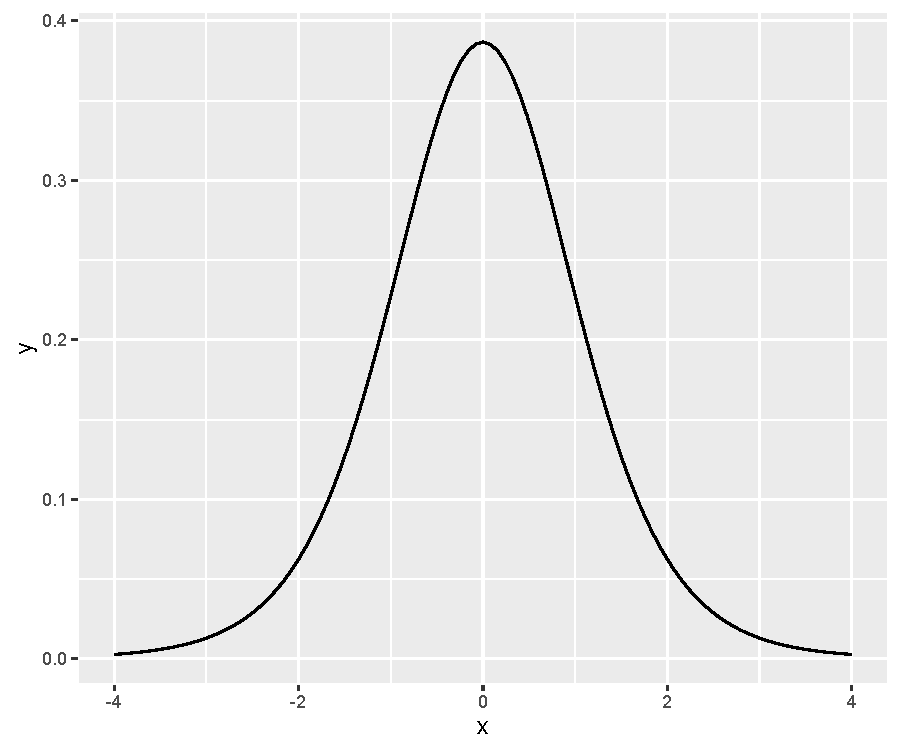
\includegraphics[width=0.6\linewidth]{9_Function_Plots_pdf/function_2-1} \end{center}

\section{Plotting your own function}\label{plotting-your-own-function}

You can also draw your own function, as long as it takes the form of a
formula that converts an x-value into a y-value. Here we have plotted a
curve that returns y-values that are the cube of x times a half:

\begin{Shaded}
\begin{Highlighting}[]
\NormalTok{cubeFun <-}\StringTok{ }\NormalTok{function(x) \{}
    \NormalTok{x^}\DecValTok{3} \NormalTok{*}\StringTok{ }\FloatTok{0.5}
\NormalTok{\}}

\NormalTok{p9 <-}\StringTok{ }\KeywordTok{ggplot}\NormalTok{(}\KeywordTok{data.frame}\NormalTok{(}\DataTypeTok{x =} \KeywordTok{c}\NormalTok{(-}\DecValTok{4}\NormalTok{, }\DecValTok{4}\NormalTok{)), }\KeywordTok{aes}\NormalTok{(}\DataTypeTok{x =} \NormalTok{x)) +}
\StringTok{  }\KeywordTok{stat_function}\NormalTok{(}\DataTypeTok{fun =} \NormalTok{cubeFun)}
\NormalTok{p9}
\end{Highlighting}
\end{Shaded}

\begin{center}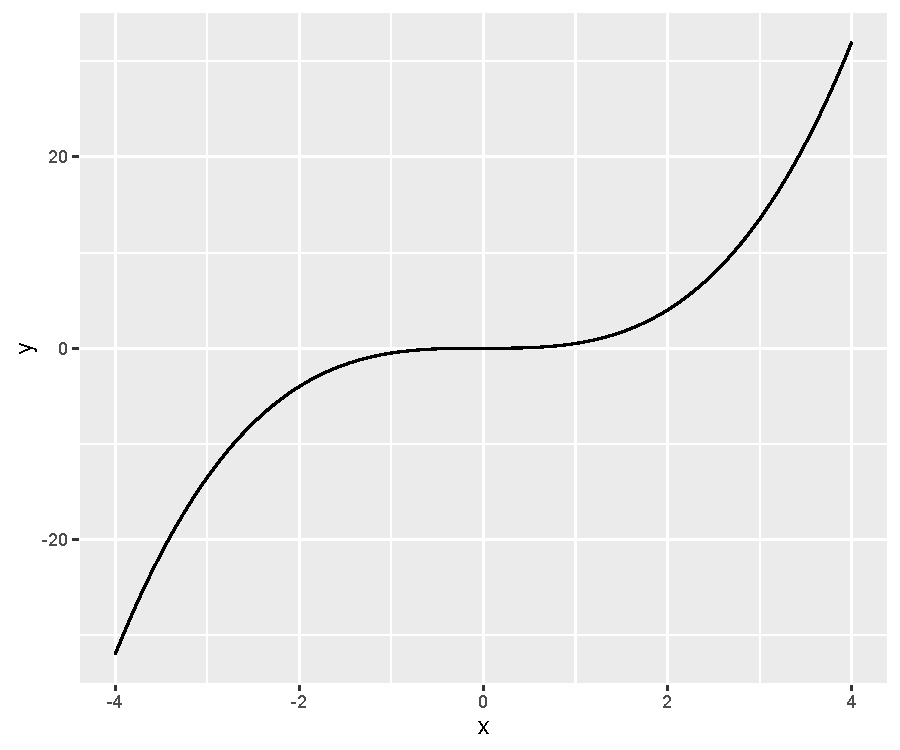
\includegraphics[width=0.6\linewidth]{9_Function_Plots_pdf/function_3-1} \end{center}

\section{Plotting multiple functions on the same
graph}\label{plotting-multiple-functions-on-the-same-graph}

You can plot multiple functions on the same graph by simply adding
another \texttt{stat\_function()} for each curve. Here we have plotted
two normal curves on the same graph, one with a mean of 0.2 and a
standard deviation of 0.1, and one with a mean of 0.7 and a standard
deviation of 0.05. (Note that the \texttt{dnorm} function has a default
mean of 0 and a default standard deviation of 1, which is why we didn't
need to explicitly define them in the first normal curve we plotted
above.) You can also see we've changed the range of the x-axis to
between 0 and 1.

\begin{Shaded}
\begin{Highlighting}[]
\NormalTok{p9 <-}\StringTok{ }\KeywordTok{ggplot}\NormalTok{(}\KeywordTok{data.frame}\NormalTok{(}\DataTypeTok{x =} \KeywordTok{c}\NormalTok{(}\DecValTok{0}\NormalTok{, }\DecValTok{1}\NormalTok{)), }\KeywordTok{aes}\NormalTok{(}\DataTypeTok{x =} \NormalTok{x)) +}
\StringTok{  }\KeywordTok{stat_function}\NormalTok{(}\DataTypeTok{fun =} \NormalTok{dnorm, }\DataTypeTok{args =} \KeywordTok{list}\NormalTok{(}\FloatTok{0.2}\NormalTok{, }\FloatTok{0.1}\NormalTok{)) +}
\StringTok{  }\KeywordTok{stat_function}\NormalTok{(}\DataTypeTok{fun =} \NormalTok{dnorm, }\DataTypeTok{args =} \KeywordTok{list}\NormalTok{(}\FloatTok{0.7}\NormalTok{, }\FloatTok{0.05}\NormalTok{))}
\NormalTok{p9}
\end{Highlighting}
\end{Shaded}

\begin{center}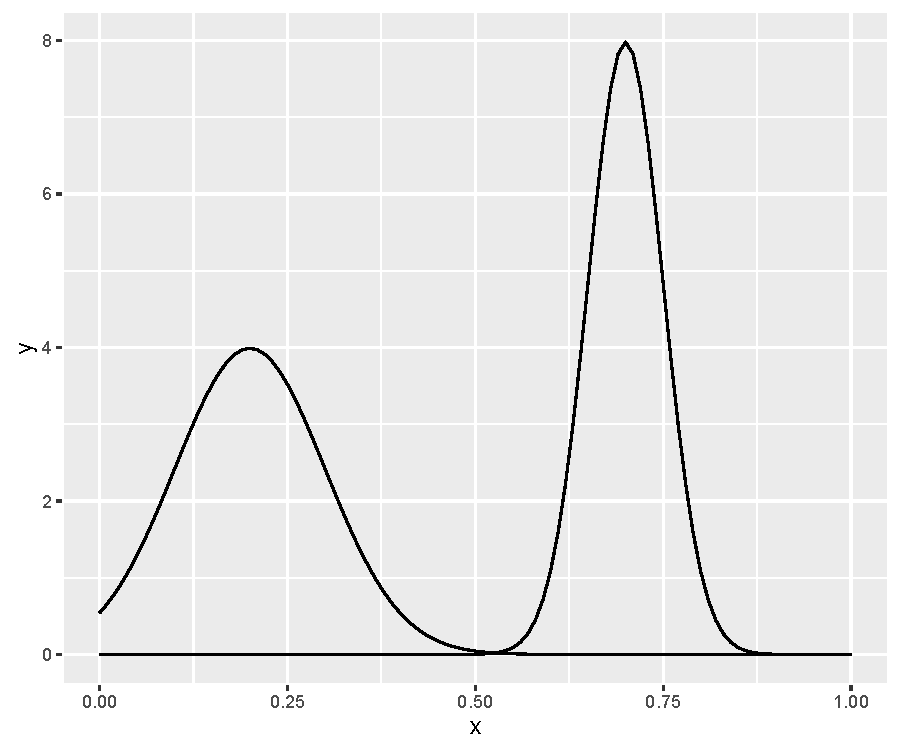
\includegraphics[width=0.6\linewidth]{9_Function_Plots_pdf/function_4-1} \end{center}

\section{Customising axis labels}\label{customising-axis-labels}

Let's move forward with this two function graph, and start tweaking the
appearance. In order to change the axis labels, we have a couple of
options. In this case, we have used the \texttt{scale\_x\_continuous}
and \texttt{scale\_y\_continuous} options, as these have further
customisation options for the axes we will use below. In each, we add
the desired name to the \texttt{name} argument as a string.

\begin{Shaded}
\begin{Highlighting}[]
\NormalTok{p9 <-}\StringTok{ }\NormalTok{p9 +}\StringTok{ }\KeywordTok{scale_x_continuous}\NormalTok{(}\DataTypeTok{name =} \StringTok{"Probability"}\NormalTok{) +}
\StringTok{  }\KeywordTok{scale_y_continuous}\NormalTok{(}\DataTypeTok{name =} \StringTok{"Frequency"}\NormalTok{)}
\NormalTok{p9}
\end{Highlighting}
\end{Shaded}

\begin{center}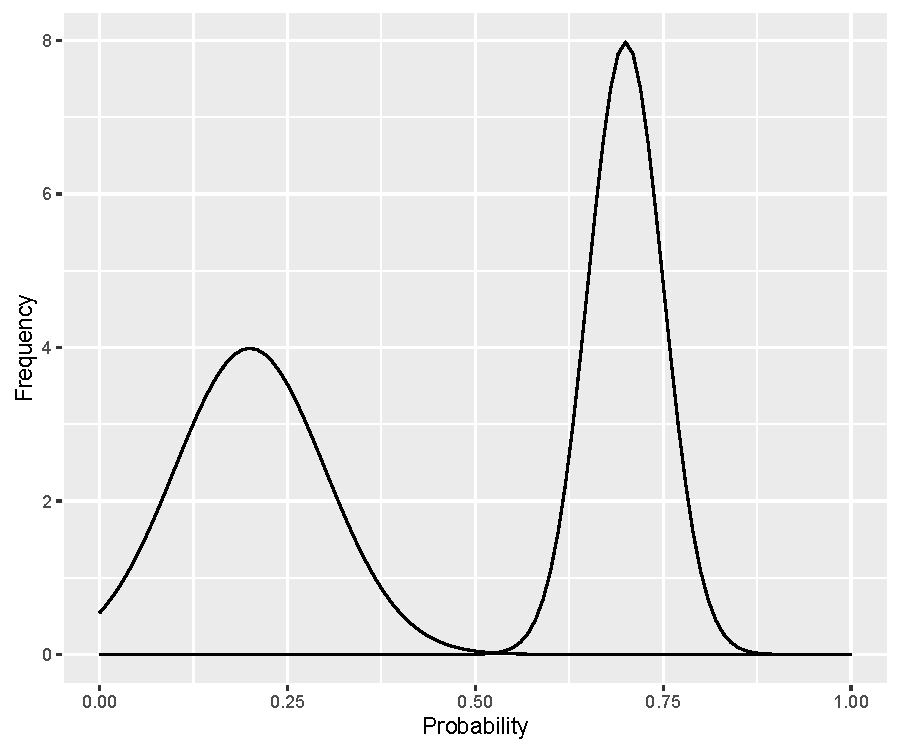
\includegraphics[width=0.6\linewidth]{9_Function_Plots_pdf/function_5-1} \end{center}

\section{Changing axis ticks}\label{changing-axis-ticks}

The next thing we will change is the axis ticks. Let's make the x-axis
ticks appear at every 0.2 units rather than 0.25 using the
\texttt{breaks\ =\ seq(0,\ 1,\ 0.2)} argument in
\texttt{scale\_x\_continuous}. (The \texttt{seq} function is a base R
function that indicates the start and endpoints and the units to
increment by respectively. See \texttt{help(seq)} for more information.)
We ensure that the x-axis begins and ends where we want by also adding
the argument \texttt{limits\ =\ c(0,\ 1)} to
\texttt{scale\_x\_continuous}.

\begin{Shaded}
\begin{Highlighting}[]
\NormalTok{p9 <-}\StringTok{ }\NormalTok{p9 +}\StringTok{ }\KeywordTok{scale_x_continuous}\NormalTok{(}\DataTypeTok{name =} \StringTok{"Probability"}\NormalTok{,}
    \DataTypeTok{breaks =} \KeywordTok{seq}\NormalTok{(}\DecValTok{0}\NormalTok{, }\DecValTok{1}\NormalTok{, }\FloatTok{0.2}\NormalTok{), }\DataTypeTok{limits=}\KeywordTok{c}\NormalTok{(}\DecValTok{0}\NormalTok{, }\DecValTok{1}\NormalTok{)) +}
\StringTok{  }\KeywordTok{scale_y_continuous}\NormalTok{(}\DataTypeTok{name =} \StringTok{"Frequency"}\NormalTok{)}
\NormalTok{p9}
\end{Highlighting}
\end{Shaded}

\begin{center}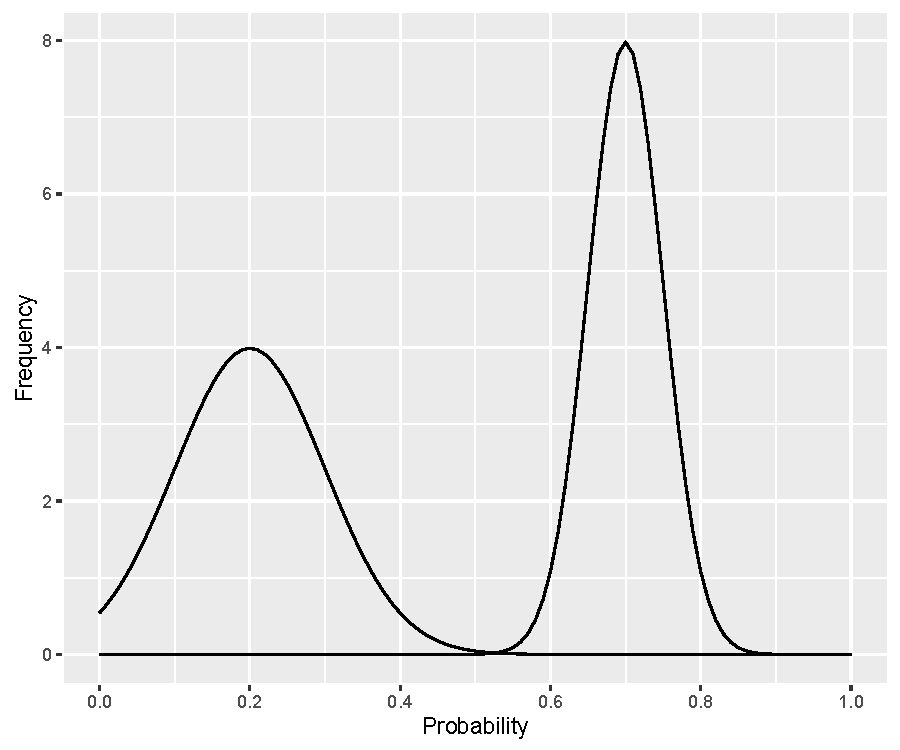
\includegraphics[width=0.6\linewidth]{9_Function_Plots_pdf/function_6-1} \end{center}

\section{Adding a title}\label{adding-a-title}

To add a title, we include the option \texttt{ggtitle} and include the
name of the graph as a string argument.

\begin{Shaded}
\begin{Highlighting}[]
\NormalTok{p9 <-}\StringTok{ }\NormalTok{p9 +}\StringTok{ }\KeywordTok{ggtitle}\NormalTok{(}\StringTok{"Normal function curves of probabilities"}\NormalTok{)}
\NormalTok{p9}
\end{Highlighting}
\end{Shaded}

\begin{center}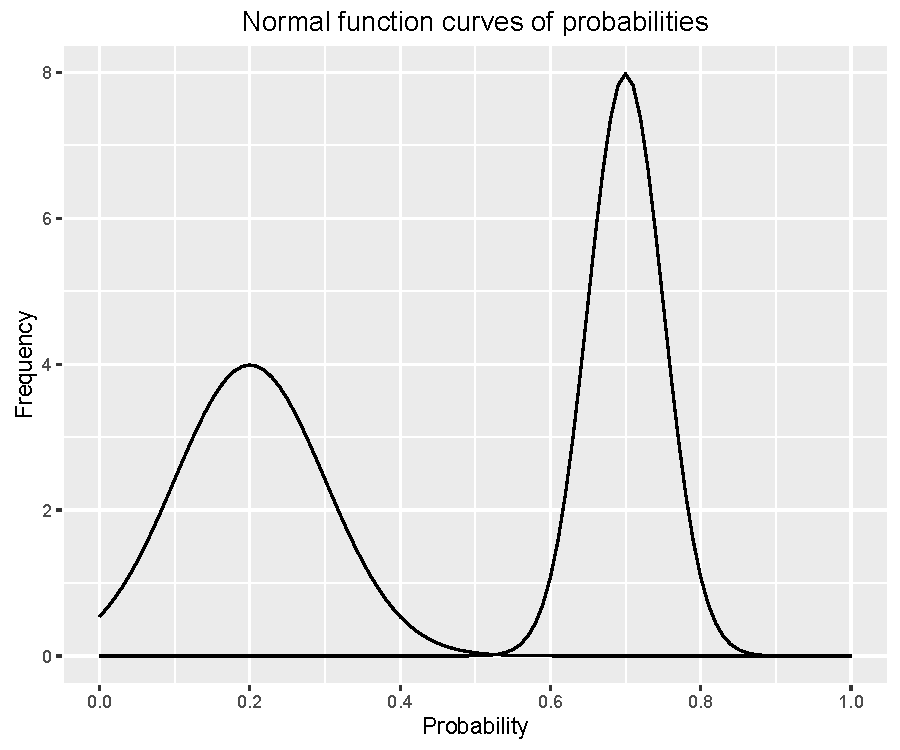
\includegraphics[width=0.6\linewidth]{9_Function_Plots_pdf/function_7-1} \end{center}

\section{Changing the colour of the
curves}\label{changing-the-colour-of-the-curves}

To change the line colours of the curves, we add a valid colour to the
\texttt{colour} arguments in \texttt{stat\_function}. A list of valid
colours is
\href{http://www.stat.columbia.edu/~tzheng/files/Rcolor.pdf}{here}.

\begin{Shaded}
\begin{Highlighting}[]
\NormalTok{p9 <-}\StringTok{ }\KeywordTok{ggplot}\NormalTok{(}\KeywordTok{data.frame}\NormalTok{(}\DataTypeTok{x =} \KeywordTok{c}\NormalTok{(}\DecValTok{0}\NormalTok{, }\DecValTok{1}\NormalTok{)), }\KeywordTok{aes}\NormalTok{(}\DataTypeTok{x =} \NormalTok{x)) +}
\StringTok{    }\KeywordTok{stat_function}\NormalTok{(}\DataTypeTok{fun =} \NormalTok{dnorm, }\DataTypeTok{args =} \KeywordTok{list}\NormalTok{(}\FloatTok{0.2}\NormalTok{, }\FloatTok{0.1}\NormalTok{),}
      \DataTypeTok{colour =} \StringTok{"deeppink"}\NormalTok{) +}
\StringTok{    }\KeywordTok{stat_function}\NormalTok{(}\DataTypeTok{fun =} \NormalTok{dnorm, }\DataTypeTok{args =} \KeywordTok{list}\NormalTok{(}\FloatTok{0.7}\NormalTok{, }\FloatTok{0.05}\NormalTok{),}
      \DataTypeTok{colour =} \StringTok{"dodgerblue3"}\NormalTok{) +}
\StringTok{    }\KeywordTok{scale_x_continuous}\NormalTok{(}\DataTypeTok{name =} \StringTok{"Probability"}\NormalTok{,}
      \DataTypeTok{breaks =} \KeywordTok{seq}\NormalTok{(}\DecValTok{0}\NormalTok{, }\DecValTok{1}\NormalTok{, }\FloatTok{0.2}\NormalTok{), }\DataTypeTok{limits=}\KeywordTok{c}\NormalTok{(}\DecValTok{0}\NormalTok{, }\DecValTok{1}\NormalTok{)) +}
\StringTok{    }\KeywordTok{scale_y_continuous}\NormalTok{(}\DataTypeTok{name =} \StringTok{"Frequency"}\NormalTok{) +}
\StringTok{    }\KeywordTok{ggtitle}\NormalTok{(}\StringTok{"Normal function curves of probabilities"}\NormalTok{)}
\NormalTok{p9}
\end{Highlighting}
\end{Shaded}

\begin{center}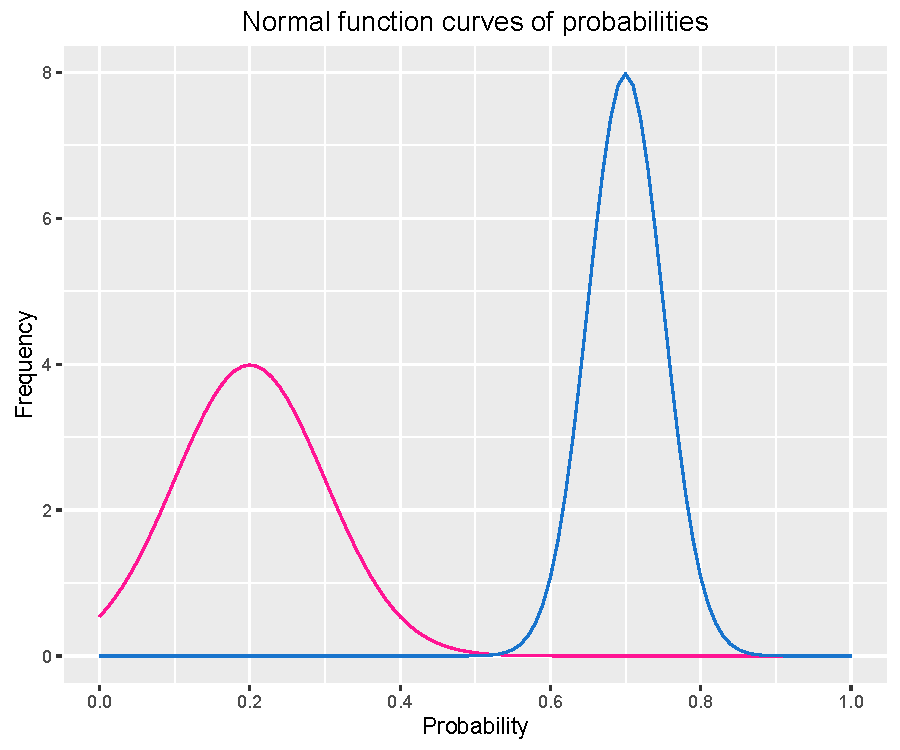
\includegraphics[width=0.6\linewidth]{9_Function_Plots_pdf/function_8-1} \end{center}

If you want to go beyond the options in the list above, you can also
specify exact HEX colours by including them as a string preceded by a
hash, e.g., ``\#FFFFFF''. Below, we have called two shades of blue for
the lines using their HEX codes.

\begin{Shaded}
\begin{Highlighting}[]
\NormalTok{p9 <-}\StringTok{ }\KeywordTok{ggplot}\NormalTok{(}\KeywordTok{data.frame}\NormalTok{(}\DataTypeTok{x =} \KeywordTok{c}\NormalTok{(}\DecValTok{0}\NormalTok{, }\DecValTok{1}\NormalTok{)), }\KeywordTok{aes}\NormalTok{(}\DataTypeTok{x =} \NormalTok{x)) +}
\StringTok{    }\KeywordTok{stat_function}\NormalTok{(}\DataTypeTok{fun =} \NormalTok{dnorm, }\DataTypeTok{args =} \KeywordTok{list}\NormalTok{(}\FloatTok{0.2}\NormalTok{, }\FloatTok{0.1}\NormalTok{),}
      \DataTypeTok{colour =} \StringTok{"#4271AE"}\NormalTok{) +}
\StringTok{    }\KeywordTok{stat_function}\NormalTok{(}\DataTypeTok{fun =} \NormalTok{dnorm, }\DataTypeTok{args =} \KeywordTok{list}\NormalTok{(}\FloatTok{0.7}\NormalTok{, }\FloatTok{0.05}\NormalTok{),}
      \DataTypeTok{colour =} \StringTok{"#1F3552"}\NormalTok{) +}
\StringTok{    }\KeywordTok{scale_x_continuous}\NormalTok{(}\DataTypeTok{name =} \StringTok{"Probability"}\NormalTok{,}
      \DataTypeTok{breaks =} \KeywordTok{seq}\NormalTok{(}\DecValTok{0}\NormalTok{, }\DecValTok{1}\NormalTok{, }\FloatTok{0.2}\NormalTok{), }\DataTypeTok{limits=}\KeywordTok{c}\NormalTok{(}\DecValTok{0}\NormalTok{, }\DecValTok{1}\NormalTok{)) +}
\StringTok{    }\KeywordTok{scale_y_continuous}\NormalTok{(}\DataTypeTok{name =} \StringTok{"Frequency"}\NormalTok{) +}
\StringTok{    }\KeywordTok{ggtitle}\NormalTok{(}\StringTok{"Normal function curves of probabilities"}\NormalTok{)}
\NormalTok{p9}
\end{Highlighting}
\end{Shaded}

\begin{center}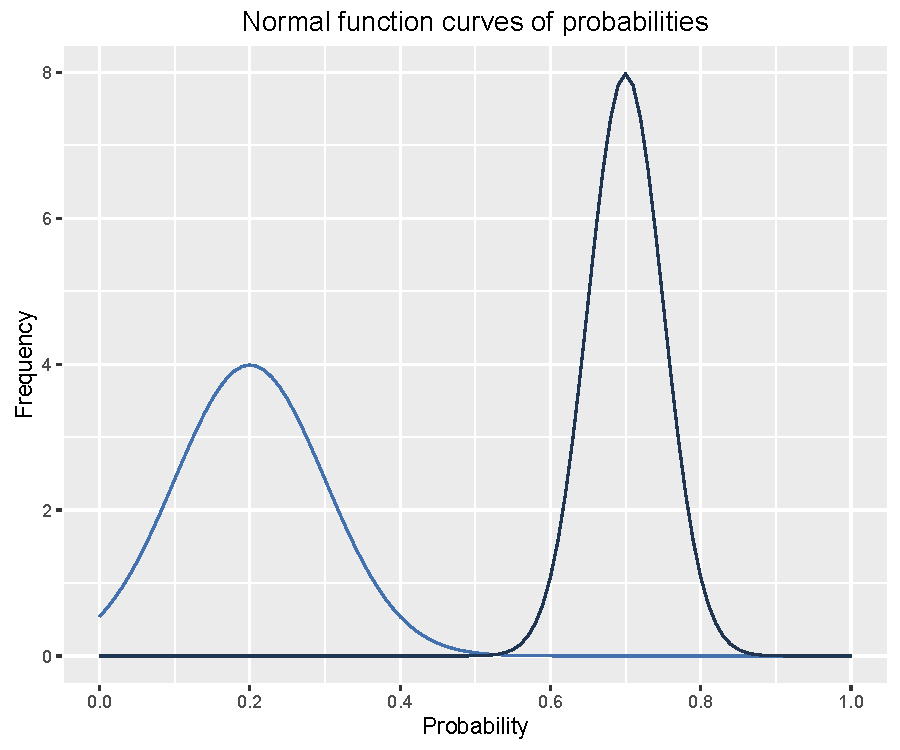
\includegraphics[width=0.6\linewidth]{9_Function_Plots_pdf/function_9-1} \end{center}

\section{Adding a legend}\label{adding-a-legend}

As we have added two separate commands to plot the two function curves,
ggplot does not automatically recognise that it needs to create a
legend. We can make a legend by swapping out the \texttt{colour}
argument in each of the \texttt{stat\_function} commands for
\texttt{aes(colour\ =\ )}, and assigning it the name of the group. We
also need to add the \texttt{scale\_colour\_manual} command to make the
legend appear, and also assign colours and a title.

\begin{Shaded}
\begin{Highlighting}[]
\NormalTok{p9 <-}\StringTok{ }\KeywordTok{ggplot}\NormalTok{(}\KeywordTok{data.frame}\NormalTok{(}\DataTypeTok{x =} \KeywordTok{c}\NormalTok{(}\DecValTok{0}\NormalTok{, }\DecValTok{1}\NormalTok{)), }\KeywordTok{aes}\NormalTok{(}\DataTypeTok{x =} \NormalTok{x)) +}
\StringTok{    }\KeywordTok{stat_function}\NormalTok{(}\DataTypeTok{fun =} \NormalTok{dnorm, }\DataTypeTok{args =} \KeywordTok{list}\NormalTok{(}\FloatTok{0.2}\NormalTok{, }\FloatTok{0.1}\NormalTok{),}
      \KeywordTok{aes}\NormalTok{(}\DataTypeTok{colour =} \StringTok{"Group 1 "}\NormalTok{)) +}
\StringTok{    }\KeywordTok{stat_function}\NormalTok{(}\DataTypeTok{fun =} \NormalTok{dnorm, }\DataTypeTok{args =} \KeywordTok{list}\NormalTok{(}\FloatTok{0.7}\NormalTok{, }\FloatTok{0.05}\NormalTok{),}
      \KeywordTok{aes}\NormalTok{(}\DataTypeTok{colour =} \StringTok{"Group 2 "}\NormalTok{)) +}
\StringTok{    }\KeywordTok{scale_x_continuous}\NormalTok{(}\DataTypeTok{name =} \StringTok{"Probability"}\NormalTok{,}
      \DataTypeTok{breaks =} \KeywordTok{seq}\NormalTok{(}\DecValTok{0}\NormalTok{, }\DecValTok{1}\NormalTok{, }\FloatTok{0.2}\NormalTok{), }\DataTypeTok{limits=}\KeywordTok{c}\NormalTok{(}\DecValTok{0}\NormalTok{, }\DecValTok{1}\NormalTok{)) +}
\StringTok{    }\KeywordTok{scale_y_continuous}\NormalTok{(}\DataTypeTok{name =} \StringTok{"Frequency"}\NormalTok{) +}
\StringTok{    }\KeywordTok{ggtitle}\NormalTok{(}\StringTok{"Normal function curves of probabilities"}\NormalTok{) +}
\StringTok{    }\KeywordTok{scale_colour_manual}\NormalTok{(}\StringTok{"Groups "}\NormalTok{, }\DataTypeTok{values =} \KeywordTok{c}\NormalTok{(}\StringTok{"deeppink"}\NormalTok{, }\StringTok{"dodgerblue3"}\NormalTok{))}
\NormalTok{p9}
\end{Highlighting}
\end{Shaded}

\begin{center}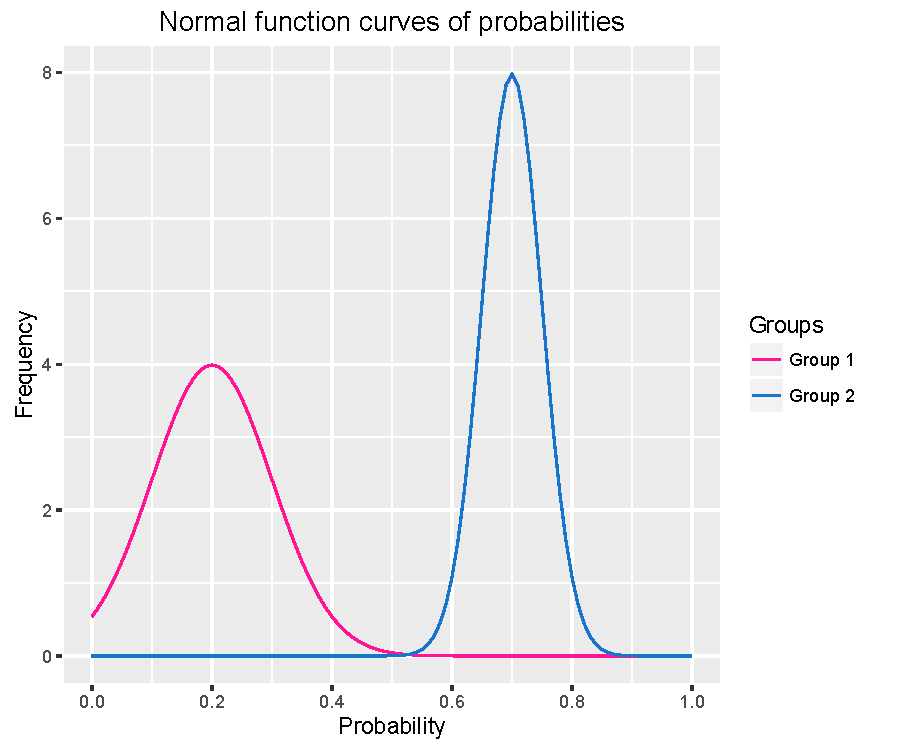
\includegraphics[width=0.6\linewidth]{9_Function_Plots_pdf/function_10-1} \end{center}

If you want to use one of the automatic brewer palettes, you can swap
\texttt{scale\_colour\_manual} for \texttt{scale\_colour\_brewer}, and
call your favouite brewer colour scheme. You can see all of the brewer
palettes using \texttt{display.brewer.all(5)} As this command doesn't
allow you to assign a title to the legend, you can assign a title using
\texttt{labs(colour\ =\ "Groups\ ")}.

\begin{Shaded}
\begin{Highlighting}[]
\NormalTok{p9 <-}\StringTok{ }\KeywordTok{ggplot}\NormalTok{(}\KeywordTok{data.frame}\NormalTok{(}\DataTypeTok{x =} \KeywordTok{c}\NormalTok{(}\DecValTok{0}\NormalTok{, }\DecValTok{1}\NormalTok{)), }\KeywordTok{aes}\NormalTok{(}\DataTypeTok{x =} \NormalTok{x)) +}
\StringTok{    }\KeywordTok{stat_function}\NormalTok{(}\DataTypeTok{fun =} \NormalTok{dnorm, }\DataTypeTok{args =} \KeywordTok{list}\NormalTok{(}\FloatTok{0.2}\NormalTok{, }\FloatTok{0.1}\NormalTok{),}
      \KeywordTok{aes}\NormalTok{(}\DataTypeTok{colour =} \StringTok{"Group 1 "}\NormalTok{)) +}
\StringTok{    }\KeywordTok{stat_function}\NormalTok{(}\DataTypeTok{fun =} \NormalTok{dnorm, }\DataTypeTok{args =} \KeywordTok{list}\NormalTok{(}\FloatTok{0.7}\NormalTok{, }\FloatTok{0.05}\NormalTok{),}
      \KeywordTok{aes}\NormalTok{(}\DataTypeTok{colour =} \StringTok{"Group 2 "}\NormalTok{)) +}
\StringTok{    }\KeywordTok{scale_x_continuous}\NormalTok{(}\DataTypeTok{name =} \StringTok{"Probability"}\NormalTok{,}
      \DataTypeTok{breaks =} \KeywordTok{seq}\NormalTok{(}\DecValTok{0}\NormalTok{, }\DecValTok{1}\NormalTok{, }\FloatTok{0.2}\NormalTok{), }\DataTypeTok{limits=}\KeywordTok{c}\NormalTok{(}\DecValTok{0}\NormalTok{, }\DecValTok{1}\NormalTok{)) +}
\StringTok{    }\KeywordTok{scale_y_continuous}\NormalTok{(}\DataTypeTok{name =} \StringTok{"Frequency"}\NormalTok{) +}
\StringTok{    }\KeywordTok{ggtitle}\NormalTok{(}\StringTok{"Normal function curves of probabilities"}\NormalTok{) +}
\StringTok{    }\KeywordTok{scale_colour_brewer}\NormalTok{(}\DataTypeTok{palette=}\StringTok{"Accent"}\NormalTok{) +}
\StringTok{    }\KeywordTok{labs}\NormalTok{(}\DataTypeTok{colour =} \StringTok{"Groups "}\NormalTok{)}
\NormalTok{p9}
\end{Highlighting}
\end{Shaded}

\begin{center}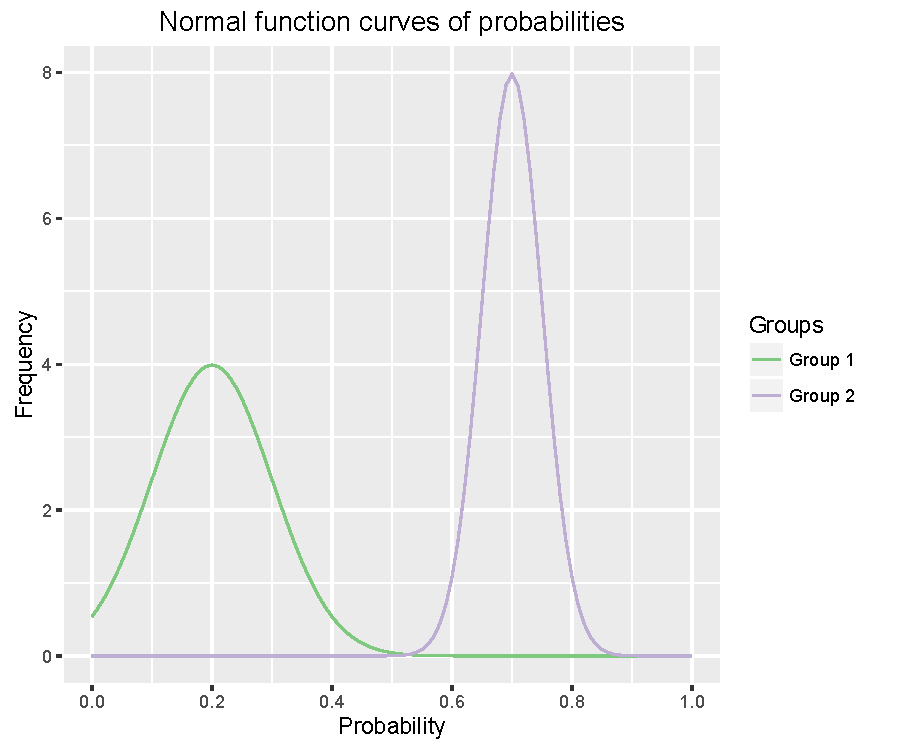
\includegraphics[width=0.6\linewidth]{9_Function_Plots_pdf/function_11-1} \end{center}

\section{Changing the size of the
lines}\label{changing-the-size-of-the-lines}

As you can see, the lines are a little difficult to see. You can make
them thicker (or thinner) using the argument \texttt{size} argument
within \texttt{stat\_function}. Here we have changed the thickness of
each line to size 2.

\begin{Shaded}
\begin{Highlighting}[]
\NormalTok{p9 <-}\StringTok{ }\KeywordTok{ggplot}\NormalTok{(}\KeywordTok{data.frame}\NormalTok{(}\DataTypeTok{x =} \KeywordTok{c}\NormalTok{(}\DecValTok{0}\NormalTok{, }\DecValTok{1}\NormalTok{)), }\KeywordTok{aes}\NormalTok{(}\DataTypeTok{x =} \NormalTok{x)) +}
\StringTok{    }\KeywordTok{stat_function}\NormalTok{(}\DataTypeTok{fun =} \NormalTok{dnorm, }\DataTypeTok{args =} \KeywordTok{list}\NormalTok{(}\FloatTok{0.2}\NormalTok{, }\FloatTok{0.1}\NormalTok{),}
      \KeywordTok{aes}\NormalTok{(}\DataTypeTok{colour =} \StringTok{"Group 1 "}\NormalTok{), }\DataTypeTok{size =} \FloatTok{1.5}\NormalTok{) +}
\StringTok{    }\KeywordTok{stat_function}\NormalTok{(}\DataTypeTok{fun =} \NormalTok{dnorm, }\DataTypeTok{args =} \KeywordTok{list}\NormalTok{(}\FloatTok{0.7}\NormalTok{, }\FloatTok{0.05}\NormalTok{),}
      \KeywordTok{aes}\NormalTok{(}\DataTypeTok{colour =} \StringTok{"Group 2 "}\NormalTok{), }\DataTypeTok{size =} \FloatTok{1.5}\NormalTok{) +}
\StringTok{    }\KeywordTok{scale_x_continuous}\NormalTok{(}\DataTypeTok{name =} \StringTok{"Probability"}\NormalTok{,}
      \DataTypeTok{breaks =} \KeywordTok{seq}\NormalTok{(}\DecValTok{0}\NormalTok{, }\DecValTok{1}\NormalTok{, }\FloatTok{0.2}\NormalTok{), }\DataTypeTok{limits=}\KeywordTok{c}\NormalTok{(}\DecValTok{0}\NormalTok{, }\DecValTok{1}\NormalTok{)) +}
\StringTok{    }\KeywordTok{scale_y_continuous}\NormalTok{(}\DataTypeTok{name =} \StringTok{"Frequency"}\NormalTok{) +}
\StringTok{    }\KeywordTok{ggtitle}\NormalTok{(}\StringTok{"Normal function curves of probabilities"}\NormalTok{) +}
\StringTok{    }\KeywordTok{scale_colour_brewer}\NormalTok{(}\DataTypeTok{palette=}\StringTok{"Accent"}\NormalTok{) +}
\StringTok{    }\KeywordTok{labs}\NormalTok{(}\DataTypeTok{colour =} \StringTok{"Groups "}\NormalTok{)}
\NormalTok{p9}
\end{Highlighting}
\end{Shaded}

\begin{center}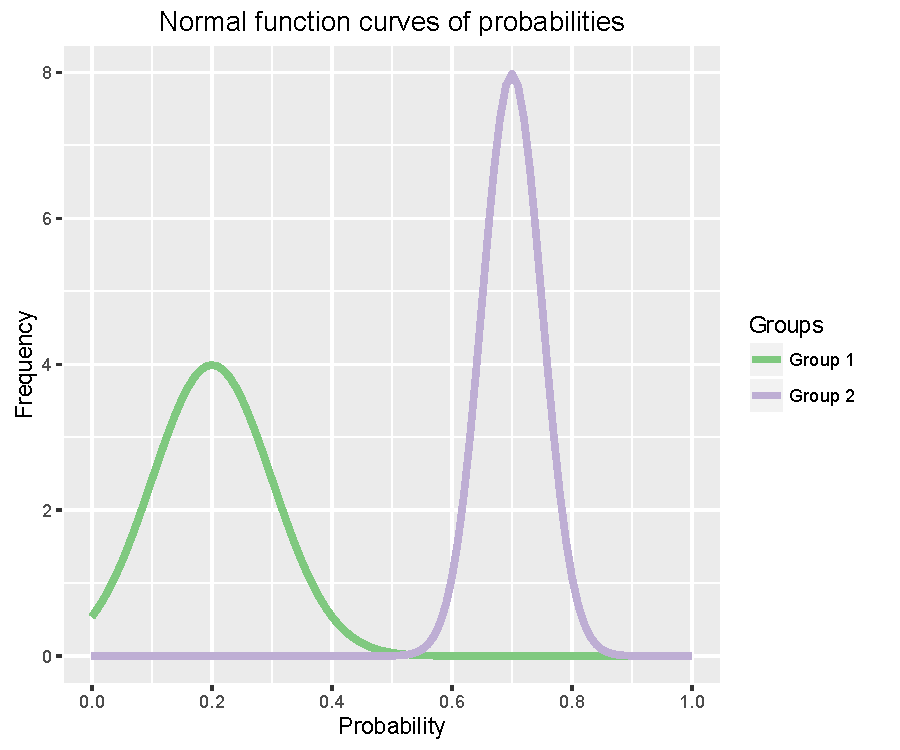
\includegraphics[width=0.6\linewidth]{9_Function_Plots_pdf/function_12-1} \end{center}

\section{Using the white theme}\label{using-the-white-theme}

As explained in the previous posts, we can also change the overall look
of the plot using themes. We'll start using a simple theme customisation
by adding \texttt{theme\_bw()} after \texttt{ggplot()}. As you can see,
we can further tweak the graph using the \texttt{theme} option, which
we've used so far to change the legend.

\begin{Shaded}
\begin{Highlighting}[]
\NormalTok{p9 <-}\StringTok{ }\NormalTok{p9 +}\StringTok{ }\KeywordTok{theme_bw}\NormalTok{()}
\NormalTok{p9}
\end{Highlighting}
\end{Shaded}

\begin{center}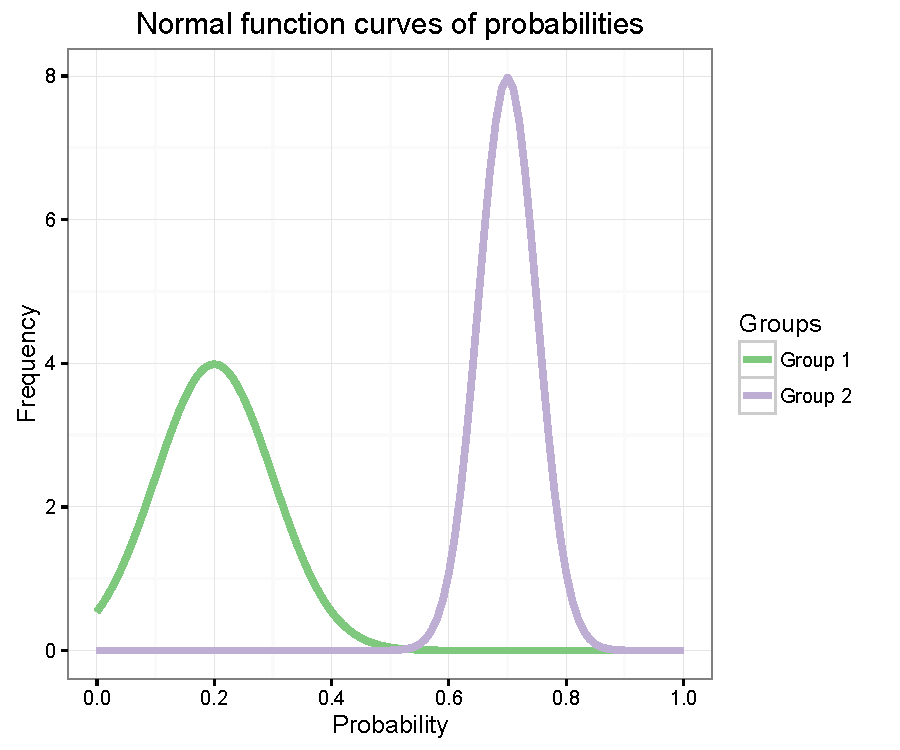
\includegraphics[width=0.6\linewidth]{9_Function_Plots_pdf/function_13-1} \end{center}

\section{Creating an XKCD style
chart}\label{creating-an-xkcd-style-chart}

Of course, you may want to create your own themes as well.
\texttt{ggplot2} allows for a very high degree of customisation,
including allowing you to use imported fonts. Below is an example of a
theme Mauricio was able to create which mimics the visual style of
\href{http://xkcd.com/}{XKCD}. In order to create this chart, you first
need to import the XKCD font, and load it into R using the
\texttt{extrafont} package.

\begin{Shaded}
\begin{Highlighting}[]
\NormalTok{p9 <-}\StringTok{ }\KeywordTok{ggplot}\NormalTok{(}\KeywordTok{data.frame}\NormalTok{(}\DataTypeTok{x =} \KeywordTok{c}\NormalTok{(}\DecValTok{0}\NormalTok{, }\DecValTok{1}\NormalTok{)), }\KeywordTok{aes}\NormalTok{(}\DataTypeTok{x =} \NormalTok{x)) +}
\StringTok{  }\KeywordTok{stat_function}\NormalTok{(}\DataTypeTok{fun =} \NormalTok{dnorm, }\DataTypeTok{args =} \KeywordTok{list}\NormalTok{(}\FloatTok{0.2}\NormalTok{, }\FloatTok{0.1}\NormalTok{),}
    \KeywordTok{aes}\NormalTok{(}\DataTypeTok{colour =} \StringTok{"Group 1 "}\NormalTok{), }\DataTypeTok{size =} \FloatTok{1.5}\NormalTok{) +}
\StringTok{  }\KeywordTok{stat_function}\NormalTok{(}\DataTypeTok{fun =} \NormalTok{dnorm, }\DataTypeTok{args =} \KeywordTok{list}\NormalTok{(}\FloatTok{0.7}\NormalTok{, }\FloatTok{0.05}\NormalTok{),}
    \KeywordTok{aes}\NormalTok{(}\DataTypeTok{colour =} \StringTok{"Group 2 "}\NormalTok{), }\DataTypeTok{size =} \FloatTok{1.5}\NormalTok{) +}
\StringTok{  }\KeywordTok{scale_x_continuous}\NormalTok{(}\DataTypeTok{name =} \StringTok{"Probability"}\NormalTok{,}
    \DataTypeTok{breaks =} \KeywordTok{seq}\NormalTok{(}\DecValTok{0}\NormalTok{, }\DecValTok{1}\NormalTok{, }\FloatTok{0.2}\NormalTok{), }\DataTypeTok{limits=}\KeywordTok{c}\NormalTok{(}\DecValTok{0}\NormalTok{, }\DecValTok{1}\NormalTok{)) +}
\StringTok{  }\KeywordTok{scale_y_continuous}\NormalTok{(}\DataTypeTok{name =} \StringTok{"Frequency"}\NormalTok{) +}
\StringTok{  }\KeywordTok{ggtitle}\NormalTok{(}\StringTok{"Normal function curves of probabilities"}\NormalTok{) +}
\StringTok{  }\KeywordTok{scale_colour_brewer}\NormalTok{(}\DataTypeTok{palette=}\StringTok{"Set1"}\NormalTok{) +}
\StringTok{  }\KeywordTok{labs}\NormalTok{(}\DataTypeTok{colour =} \StringTok{"Groups "}\NormalTok{) +}
\StringTok{  }\KeywordTok{theme}\NormalTok{(}\DataTypeTok{axis.line.x =} \KeywordTok{element_line}\NormalTok{(}\DataTypeTok{size=}\NormalTok{.}\DecValTok{5}\NormalTok{, }\DataTypeTok{colour =} \StringTok{"black"}\NormalTok{), }
    \DataTypeTok{axis.line.y =} \KeywordTok{element_line}\NormalTok{(}\DataTypeTok{size=}\NormalTok{.}\DecValTok{5}\NormalTok{, }\DataTypeTok{colour =} \StringTok{"black"}\NormalTok{),     }
    \DataTypeTok{axis.text.x=}\KeywordTok{element_text}\NormalTok{(}\DataTypeTok{colour=}\StringTok{"black"}\NormalTok{, }\DataTypeTok{size =} \DecValTok{10}\NormalTok{), }
    \DataTypeTok{axis.text.y=}\KeywordTok{element_text}\NormalTok{(}\DataTypeTok{colour=}\StringTok{"black"}\NormalTok{, }\DataTypeTok{size =} \DecValTok{10}\NormalTok{), }
    \DataTypeTok{legend.position=}\StringTok{"bottom"}\NormalTok{, }
    \DataTypeTok{legend.direction=}\StringTok{"horizontal"}\NormalTok{,}
    \DataTypeTok{legend.box =} \StringTok{"horizontal"}\NormalTok{, }
    \DataTypeTok{legend.key =} \KeywordTok{element_blank}\NormalTok{(),}
    \DataTypeTok{panel.grid.major =} \KeywordTok{element_blank}\NormalTok{(),}
    \DataTypeTok{panel.grid.minor =} \KeywordTok{element_blank}\NormalTok{(), }
    \DataTypeTok{panel.border =} \KeywordTok{element_blank}\NormalTok{(),}
    \DataTypeTok{panel.background =} \KeywordTok{element_blank}\NormalTok{(),}
    \DataTypeTok{plot.title=}\KeywordTok{element_text}\NormalTok{(}\DataTypeTok{family=}\StringTok{"xkcd-Regular"}\NormalTok{), }
    \DataTypeTok{text=}\KeywordTok{element_text}\NormalTok{(}\DataTypeTok{family=}\StringTok{"xkcd-Regular"}\NormalTok{)) }
\NormalTok{p9}
\end{Highlighting}
\end{Shaded}

\begin{center}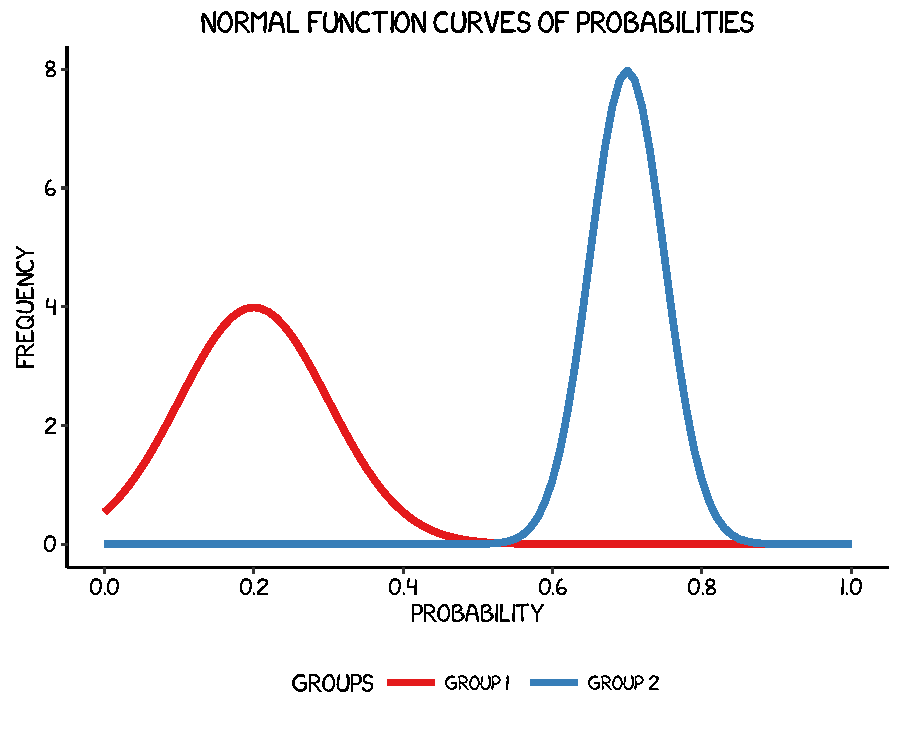
\includegraphics[width=0.6\linewidth]{9_Function_Plots_pdf/function_14-1} \end{center}

\section{\texorpdfstring{Using `The Economist'
theme}{Using The Economist theme}}\label{using-the-economist-theme}

There are a wider range of pre-built themes available as part of the
\texttt{ggthemes} package (more information on these
\href{https://cran.r-project.org/web/packages/ggthemes/vignettes/ggthemes.html}{here}).
Below we've applied \texttt{theme\_economist()}, which approximates
graphs in the Economist magazine.

\begin{Shaded}
\begin{Highlighting}[]
\NormalTok{p9 <-}\StringTok{ }\KeywordTok{ggplot}\NormalTok{(}\KeywordTok{data.frame}\NormalTok{(}\DataTypeTok{x =} \KeywordTok{c}\NormalTok{(}\DecValTok{0}\NormalTok{, }\DecValTok{1}\NormalTok{)), }\KeywordTok{aes}\NormalTok{(}\DataTypeTok{x =} \NormalTok{x)) +}
\StringTok{  }\KeywordTok{stat_function}\NormalTok{(}\DataTypeTok{fun =} \NormalTok{dnorm, }\DataTypeTok{args =} \KeywordTok{list}\NormalTok{(}\FloatTok{0.2}\NormalTok{, }\FloatTok{0.1}\NormalTok{),}
    \KeywordTok{aes}\NormalTok{(}\DataTypeTok{colour =} \StringTok{"Group 1 "}\NormalTok{), }\DataTypeTok{size =} \FloatTok{1.5}\NormalTok{) +}
\StringTok{  }\KeywordTok{stat_function}\NormalTok{(}\DataTypeTok{fun =} \NormalTok{dnorm, }\DataTypeTok{args =} \KeywordTok{list}\NormalTok{(}\FloatTok{0.7}\NormalTok{, }\FloatTok{0.05}\NormalTok{),}
    \KeywordTok{aes}\NormalTok{(}\DataTypeTok{colour =} \StringTok{"Group 2 "}\NormalTok{), }\DataTypeTok{size =} \FloatTok{1.5}\NormalTok{) +}
\StringTok{  }\KeywordTok{scale_x_continuous}\NormalTok{(}\DataTypeTok{name =} \StringTok{"Probability"}\NormalTok{,}
    \DataTypeTok{breaks =} \KeywordTok{seq}\NormalTok{(}\DecValTok{0}\NormalTok{, }\DecValTok{1}\NormalTok{, }\FloatTok{0.2}\NormalTok{), }\DataTypeTok{limits=}\KeywordTok{c}\NormalTok{(}\DecValTok{0}\NormalTok{, }\DecValTok{1}\NormalTok{)) +}
\StringTok{  }\KeywordTok{scale_y_continuous}\NormalTok{(}\DataTypeTok{name =} \StringTok{"Frequency"}\NormalTok{) +}
\StringTok{  }\KeywordTok{ggtitle}\NormalTok{(}\StringTok{"Normal function curves of probabilities"}\NormalTok{) +}
\StringTok{  }\KeywordTok{scale_colour_manual}\NormalTok{(}\StringTok{"Groups "}\NormalTok{, }\DataTypeTok{values =} \KeywordTok{c}\NormalTok{(}\StringTok{"#4271AE"}\NormalTok{, }\StringTok{"#1F3552"}\NormalTok{)) +}
\StringTok{  }\KeywordTok{theme_economist}\NormalTok{() +}\StringTok{ }\KeywordTok{scale_fill_economist}\NormalTok{() +}
\StringTok{  }\KeywordTok{theme}\NormalTok{(}\DataTypeTok{axis.line.x =} \KeywordTok{element_line}\NormalTok{(}\DataTypeTok{size=}\NormalTok{.}\DecValTok{5}\NormalTok{, }\DataTypeTok{colour =} \StringTok{"black"}\NormalTok{),}
    \DataTypeTok{axis.title =} \KeywordTok{element_text}\NormalTok{(}\DataTypeTok{size =} \DecValTok{12}\NormalTok{),}
    \DataTypeTok{legend.position=}\StringTok{"bottom"}\NormalTok{, }
    \DataTypeTok{legend.direction=}\StringTok{"horizontal"}\NormalTok{,}
    \DataTypeTok{legend.box =} \StringTok{"horizontal"}\NormalTok{, }
    \DataTypeTok{legend.text =} \KeywordTok{element_text}\NormalTok{(}\DataTypeTok{size =} \DecValTok{10}\NormalTok{),}
    \DataTypeTok{text =} \KeywordTok{element_text}\NormalTok{(}\DataTypeTok{family =} \StringTok{"OfficinaSanITC-Book"}\NormalTok{),}
    \DataTypeTok{plot.title =} \KeywordTok{element_text}\NormalTok{(}\DataTypeTok{family=}\StringTok{"OfficinaSanITC-Book"}\NormalTok{))}
\NormalTok{p9}
\end{Highlighting}
\end{Shaded}

\begin{center}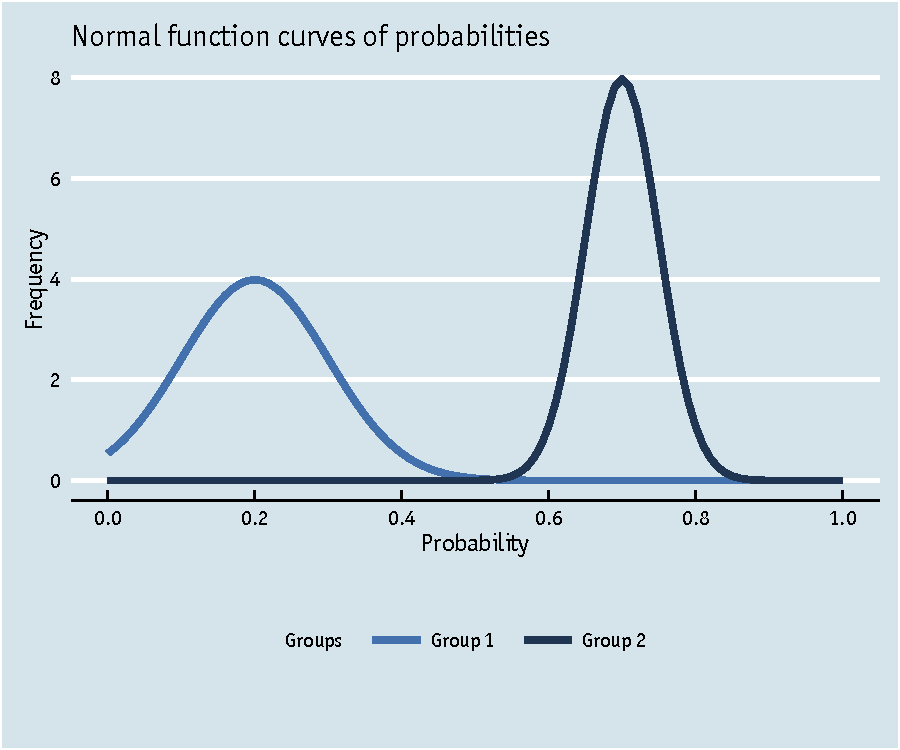
\includegraphics[width=0.6\linewidth]{9_Function_Plots_pdf/function_15-1} \end{center}

\section{\texorpdfstring{Using `Five Thirty Eight'
theme}{Using Five Thirty Eight theme}}\label{using-five-thirty-eight-theme}

Below we've applied \texttt{theme\_fivethirtyeight()}, which
approximates graphs in the nice
\href{http://fivethirtyeight.com/}{FiveThirtyEight} website. Again, it
is also important that the font change is optional and it's only to
obtain a more similar result compared to the original. For an exact
result you need `Atlas Grotesk' and `Decima Mono Pro' which are
commercial font and are available
\href{https://commercialtype.com/catalog/atlas}{here} and
\href{https://www.myfonts.com/fonts/tipografiaramis/decima-mono-pro/}{here}.

\begin{Shaded}
\begin{Highlighting}[]
\NormalTok{p9 <-}\StringTok{ }\KeywordTok{ggplot}\NormalTok{(}\KeywordTok{data.frame}\NormalTok{(}\DataTypeTok{x =} \KeywordTok{c}\NormalTok{(}\DecValTok{0}\NormalTok{, }\DecValTok{1}\NormalTok{)), }\KeywordTok{aes}\NormalTok{(}\DataTypeTok{x =} \NormalTok{x)) +}
\StringTok{  }\KeywordTok{stat_function}\NormalTok{(}\DataTypeTok{fun =} \NormalTok{dnorm, }\DataTypeTok{args =} \KeywordTok{list}\NormalTok{(}\FloatTok{0.2}\NormalTok{, }\FloatTok{0.1}\NormalTok{),}
    \KeywordTok{aes}\NormalTok{(}\DataTypeTok{colour =} \StringTok{"Group 1 "}\NormalTok{), }\DataTypeTok{size =} \FloatTok{1.5}\NormalTok{) +}
\StringTok{  }\KeywordTok{stat_function}\NormalTok{(}\DataTypeTok{fun =} \NormalTok{dnorm, }\DataTypeTok{args =} \KeywordTok{list}\NormalTok{(}\FloatTok{0.7}\NormalTok{, }\FloatTok{0.05}\NormalTok{),}
    \KeywordTok{aes}\NormalTok{(}\DataTypeTok{colour =} \StringTok{"Group 2 "}\NormalTok{), }\DataTypeTok{size =} \FloatTok{1.5}\NormalTok{) +}
\StringTok{  }\KeywordTok{scale_x_continuous}\NormalTok{(}\DataTypeTok{name =} \StringTok{"Probability"}\NormalTok{,}
    \DataTypeTok{breaks =} \KeywordTok{seq}\NormalTok{(}\DecValTok{0}\NormalTok{, }\DecValTok{1}\NormalTok{, }\FloatTok{0.2}\NormalTok{), }\DataTypeTok{limits=}\KeywordTok{c}\NormalTok{(}\DecValTok{0}\NormalTok{, }\DecValTok{1}\NormalTok{)) +}
\StringTok{  }\KeywordTok{scale_y_continuous}\NormalTok{(}\DataTypeTok{name =} \StringTok{"Frequency"}\NormalTok{) +}
\StringTok{  }\KeywordTok{ggtitle}\NormalTok{(}\StringTok{"Normal function curves of probabilities"}\NormalTok{) +}
\StringTok{  }\KeywordTok{scale_colour_manual}\NormalTok{(}\StringTok{"Groups "}\NormalTok{, }\DataTypeTok{values =} \KeywordTok{c}\NormalTok{(}\StringTok{"#4271AE"}\NormalTok{, }\StringTok{"#1F3552"}\NormalTok{)) +}
\StringTok{  }\KeywordTok{theme_fivethirtyeight}\NormalTok{() +}\StringTok{ }\KeywordTok{scale_fill_fivethirtyeight}\NormalTok{() +}\StringTok{   }
\StringTok{  }\KeywordTok{theme}\NormalTok{(}\DataTypeTok{axis.title =} \KeywordTok{element_text}\NormalTok{(}\DataTypeTok{family=}\StringTok{"Atlas Grotesk Regular"}\NormalTok{),}
    \DataTypeTok{legend.position=}\StringTok{"bottom"}\NormalTok{, }
    \DataTypeTok{legend.direction=}\StringTok{"horizontal"}\NormalTok{,}
    \DataTypeTok{legend.box =} \StringTok{"horizontal"}\NormalTok{, }
    \DataTypeTok{legend.title=}\KeywordTok{element_text}\NormalTok{(}\DataTypeTok{family=}\StringTok{"Atlas Grotesk Regular"}\NormalTok{, }\DataTypeTok{size =} \DecValTok{10}\NormalTok{),}
    \DataTypeTok{legend.text=}\KeywordTok{element_text}\NormalTok{(}\DataTypeTok{family=}\StringTok{"Atlas Grotesk Regular"}\NormalTok{, }\DataTypeTok{size =} \DecValTok{10}\NormalTok{),}
    \DataTypeTok{plot.title=}\KeywordTok{element_text}\NormalTok{(}\DataTypeTok{family=}\StringTok{"Atlas Grotesk Medium"}\NormalTok{), }
    \DataTypeTok{text=}\KeywordTok{element_text}\NormalTok{(}\DataTypeTok{family=}\StringTok{"DecimaMonoPro"}\NormalTok{)) }
\NormalTok{p9}
\end{Highlighting}
\end{Shaded}

\begin{center}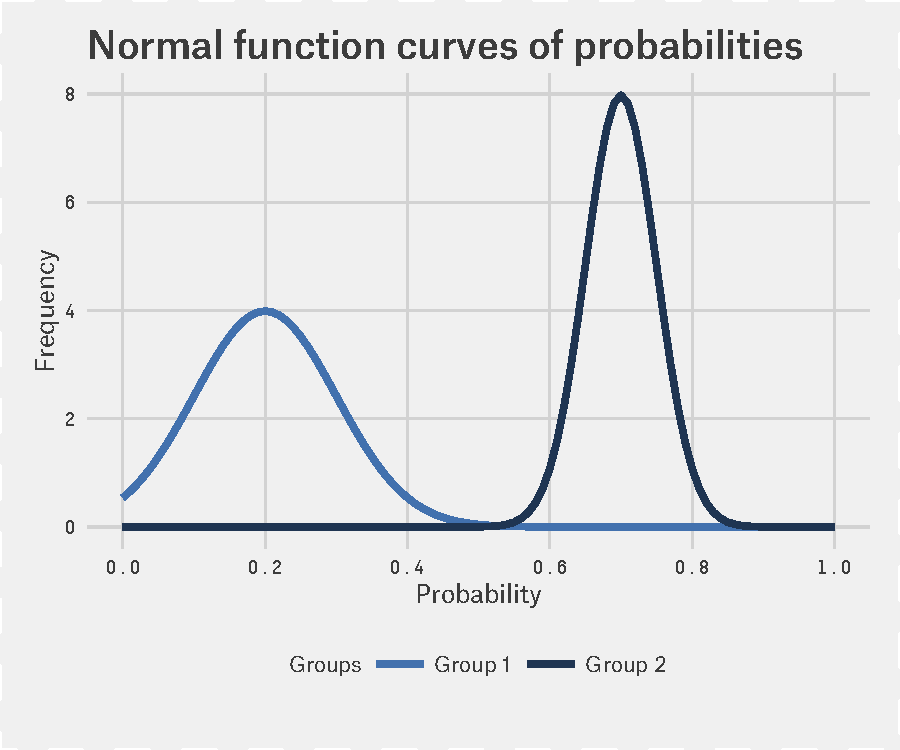
\includegraphics[width=0.6\linewidth]{9_Function_Plots_pdf/function_16-1} \end{center}

\section{Creating your own theme}\label{creating-your-own-theme}

As before, you can modify your plots a lot as \texttt{ggplot2} allows
many customisations. Here is a custom plot where we have modified the
axes, background and font.

\begin{Shaded}
\begin{Highlighting}[]
\NormalTok{p9 <-}\StringTok{ }\KeywordTok{ggplot}\NormalTok{(}\KeywordTok{data.frame}\NormalTok{(}\DataTypeTok{x =} \KeywordTok{c}\NormalTok{(}\DecValTok{0}\NormalTok{, }\DecValTok{1}\NormalTok{)), }\KeywordTok{aes}\NormalTok{(}\DataTypeTok{x =} \NormalTok{x)) +}
\StringTok{  }\KeywordTok{stat_function}\NormalTok{(}\DataTypeTok{fun =} \NormalTok{dnorm, }\DataTypeTok{args =} \KeywordTok{list}\NormalTok{(}\FloatTok{0.2}\NormalTok{, }\FloatTok{0.1}\NormalTok{),}
    \KeywordTok{aes}\NormalTok{(}\DataTypeTok{colour =} \StringTok{"Group 1 "}\NormalTok{), }\DataTypeTok{size =} \FloatTok{1.5}\NormalTok{) +}
\StringTok{  }\KeywordTok{stat_function}\NormalTok{(}\DataTypeTok{fun =} \NormalTok{dnorm, }\DataTypeTok{args =} \KeywordTok{list}\NormalTok{(}\FloatTok{0.7}\NormalTok{, }\FloatTok{0.05}\NormalTok{),}
    \KeywordTok{aes}\NormalTok{(}\DataTypeTok{colour =} \StringTok{"Group 2 "}\NormalTok{), }\DataTypeTok{size =} \FloatTok{1.5}\NormalTok{) +}
\StringTok{  }\KeywordTok{scale_x_continuous}\NormalTok{(}\DataTypeTok{name =} \StringTok{"Probability"}\NormalTok{,}
    \DataTypeTok{breaks =} \KeywordTok{seq}\NormalTok{(}\DecValTok{0}\NormalTok{, }\DecValTok{1}\NormalTok{, }\FloatTok{0.2}\NormalTok{), }\DataTypeTok{limits=}\KeywordTok{c}\NormalTok{(}\DecValTok{0}\NormalTok{, }\DecValTok{1}\NormalTok{)) +}
\StringTok{  }\KeywordTok{scale_y_continuous}\NormalTok{(}\DataTypeTok{name =} \StringTok{"Frequency"}\NormalTok{) +}
\StringTok{  }\KeywordTok{ggtitle}\NormalTok{(}\StringTok{"Normal function curves of probabilities"}\NormalTok{) +}
\StringTok{  }\KeywordTok{scale_colour_brewer}\NormalTok{(}\DataTypeTok{palette=}\StringTok{"Accent"}\NormalTok{) +}
\StringTok{  }\KeywordTok{labs}\NormalTok{(}\DataTypeTok{colour =} \StringTok{"Groups "}\NormalTok{) +}
\StringTok{  }\KeywordTok{theme_bw}\NormalTok{() +}
\StringTok{  }\KeywordTok{theme}\NormalTok{(}\DataTypeTok{panel.border =} \KeywordTok{element_rect}\NormalTok{(}\DataTypeTok{colour =} \StringTok{"black"}\NormalTok{, }\DataTypeTok{fill=}\OtherTok{NA}\NormalTok{, }\DataTypeTok{size=}\NormalTok{.}\DecValTok{5}\NormalTok{),}
    \DataTypeTok{axis.text.x=}\KeywordTok{element_text}\NormalTok{(}\DataTypeTok{colour=}\StringTok{"black"}\NormalTok{, }\DataTypeTok{size =} \DecValTok{9}\NormalTok{), }
    \DataTypeTok{axis.text.y=}\KeywordTok{element_text}\NormalTok{(}\DataTypeTok{colour=}\StringTok{"black"}\NormalTok{, }\DataTypeTok{size =} \DecValTok{9}\NormalTok{), }
    \DataTypeTok{panel.grid.major =} \KeywordTok{element_line}\NormalTok{(}\DataTypeTok{colour =} \StringTok{"#d3d3d3"}\NormalTok{), }
    \DataTypeTok{panel.grid.minor =} \KeywordTok{element_blank}\NormalTok{(), }
    \DataTypeTok{panel.border =} \KeywordTok{element_blank}\NormalTok{(), }\DataTypeTok{panel.background =} \KeywordTok{element_blank}\NormalTok{(),}
    \DataTypeTok{plot.title =} \KeywordTok{element_text}\NormalTok{(}\DataTypeTok{size =} \DecValTok{14}\NormalTok{, }\DataTypeTok{family =} \StringTok{"Tahoma"}\NormalTok{, }\DataTypeTok{face =} \StringTok{"bold"}\NormalTok{),}
    \DataTypeTok{text=}\KeywordTok{element_text}\NormalTok{(}\DataTypeTok{family=}\StringTok{"Tahoma"}\NormalTok{))}
\NormalTok{p9}
\end{Highlighting}
\end{Shaded}

\begin{center}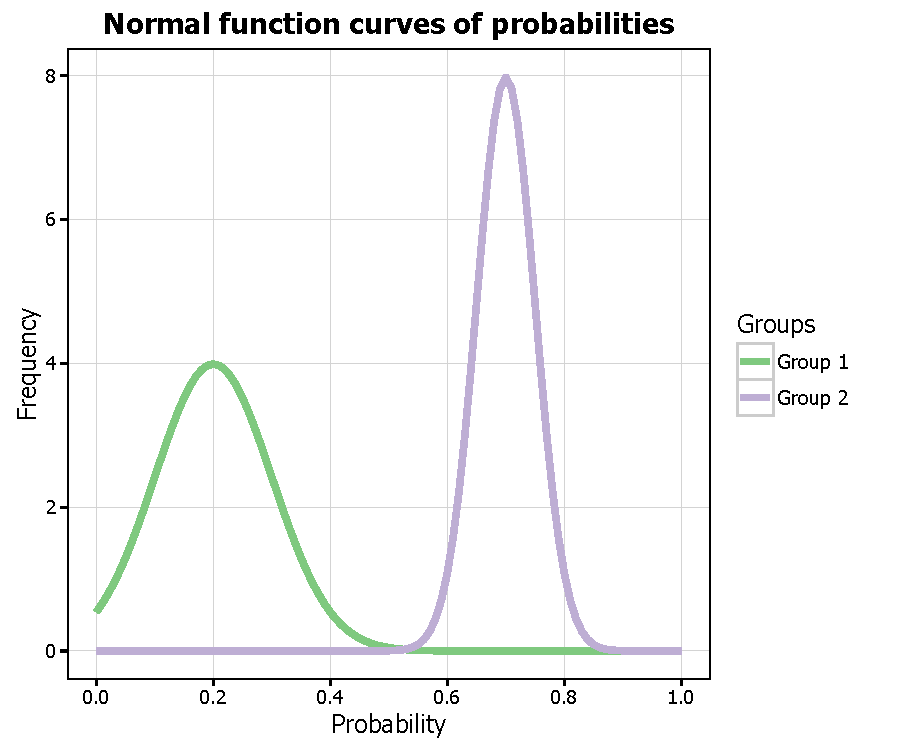
\includegraphics[width=0.6\linewidth]{9_Function_Plots_pdf/function_17-1} \end{center}

\section{Adding areas under the
curve}\label{adding-areas-under-the-curve}

If we want to shade an area under the curve, we can do so by creating a
function that generates a range of normal values with a given mean and
standard deviation, and then only retains those values that lie within
the desired range (by assigning NAs to everything outside of the range).
In this case, we have created a shaded area under the group 1 curve
which covers between the mean and 4 standard deviations above the mean
(as given by \texttt{0.2\ +\ 4\ *\ 0.1}). We then add another
\texttt{stat\_function} command to the graph which plots the area
specified by this function, indicates it should be an \texttt{area}
plot, and makes it semi-transparent using the \texttt{alpha} argument.

\begin{Shaded}
\begin{Highlighting}[]
\NormalTok{funcShaded <-}\StringTok{ }\NormalTok{function(x) \{}
    \NormalTok{y <-}\StringTok{ }\KeywordTok{dnorm}\NormalTok{(x, }\DataTypeTok{mean =} \FloatTok{0.2}\NormalTok{, }\DataTypeTok{sd =} \FloatTok{0.1}\NormalTok{)}
    \NormalTok{y[x <}\StringTok{ }\FloatTok{0.2} \NormalTok{|}\StringTok{ }\NormalTok{x >}\StringTok{ }\NormalTok{(}\FloatTok{0.2} \NormalTok{+}\StringTok{ }\DecValTok{4} \NormalTok{*}\StringTok{ }\FloatTok{0.1}\NormalTok{)] <-}\StringTok{ }\OtherTok{NA}
    \KeywordTok{return}\NormalTok{(y)}
\NormalTok{\}}

\NormalTok{p9 <-}\StringTok{ }\NormalTok{p9 +}\StringTok{ }\KeywordTok{stat_function}\NormalTok{(}\DataTypeTok{fun=}\NormalTok{funcShaded, }\DataTypeTok{geom=}\StringTok{"area"}\NormalTok{, }\DataTypeTok{fill=}\StringTok{"#84CA72"}\NormalTok{, }\DataTypeTok{alpha=}\FloatTok{0.2}\NormalTok{)}
\NormalTok{p9}
\end{Highlighting}
\end{Shaded}

\begin{center}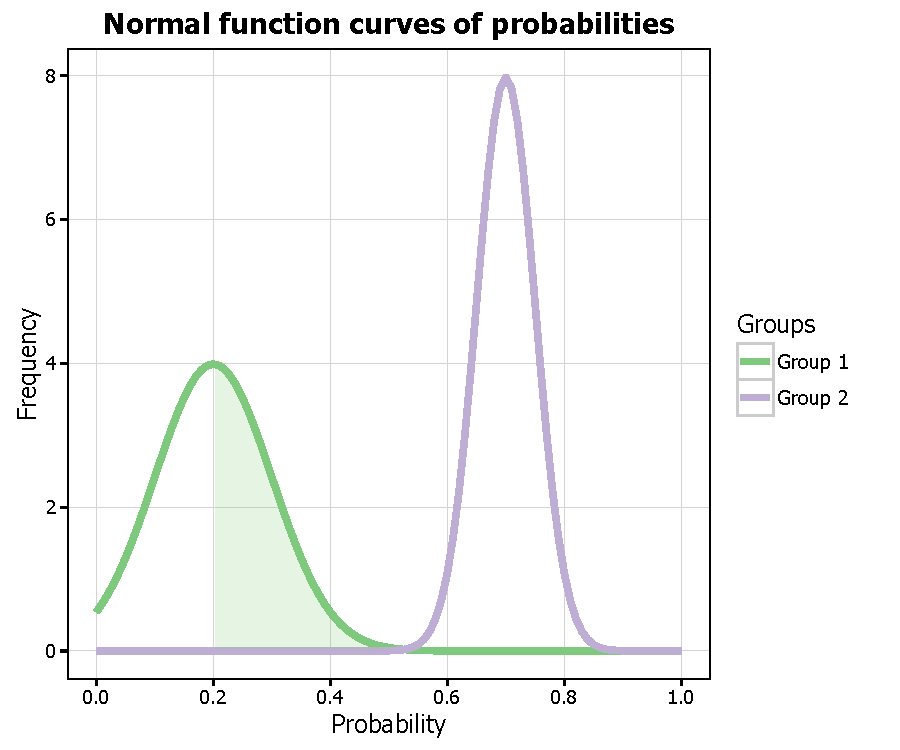
\includegraphics[width=0.6\linewidth]{9_Function_Plots_pdf/function_18-1} \end{center}

\section{Formatting the legend}\label{formatting-the-legend}

Finally, we can format the legend by changing the position. We simply
add the \texttt{legend.position\ =\ "bottom"} argument to the
\texttt{theme} option, which moves the legend under the plot.

\begin{Shaded}
\begin{Highlighting}[]
\NormalTok{p9 <-}\StringTok{ }\KeywordTok{ggplot}\NormalTok{(}\KeywordTok{data.frame}\NormalTok{(}\DataTypeTok{x =} \KeywordTok{c}\NormalTok{(}\DecValTok{0}\NormalTok{, }\DecValTok{1}\NormalTok{)), }\KeywordTok{aes}\NormalTok{(}\DataTypeTok{x =} \NormalTok{x)) +}
\StringTok{  }\KeywordTok{stat_function}\NormalTok{(}\DataTypeTok{fun =} \NormalTok{dnorm, }\DataTypeTok{args =} \KeywordTok{list}\NormalTok{(}\FloatTok{0.2}\NormalTok{, }\FloatTok{0.1}\NormalTok{),}
    \KeywordTok{aes}\NormalTok{(}\DataTypeTok{colour =} \StringTok{"Group 1 "}\NormalTok{), }\DataTypeTok{size =} \FloatTok{1.5}\NormalTok{) +}
\StringTok{  }\KeywordTok{stat_function}\NormalTok{(}\DataTypeTok{fun =} \NormalTok{dnorm, }\DataTypeTok{args =} \KeywordTok{list}\NormalTok{(}\FloatTok{0.7}\NormalTok{, }\FloatTok{0.05}\NormalTok{),}
    \KeywordTok{aes}\NormalTok{(}\DataTypeTok{colour =} \StringTok{"Group 2 "}\NormalTok{), }\DataTypeTok{size =} \FloatTok{1.5}\NormalTok{) +}
\StringTok{  }\KeywordTok{stat_function}\NormalTok{(}\DataTypeTok{fun=}\NormalTok{funcShaded, }\DataTypeTok{geom=}\StringTok{"area"}\NormalTok{, }\DataTypeTok{fill=}\StringTok{"#84CA72"}\NormalTok{, }\DataTypeTok{alpha=}\FloatTok{0.2}\NormalTok{) +}
\StringTok{  }\KeywordTok{scale_x_continuous}\NormalTok{(}\DataTypeTok{name =} \StringTok{"Probability"}\NormalTok{,}
    \DataTypeTok{breaks =} \KeywordTok{seq}\NormalTok{(}\DecValTok{0}\NormalTok{, }\DecValTok{1}\NormalTok{, }\FloatTok{0.2}\NormalTok{), }\DataTypeTok{limits=}\KeywordTok{c}\NormalTok{(}\DecValTok{0}\NormalTok{, }\DecValTok{1}\NormalTok{)) +}
\StringTok{  }\KeywordTok{scale_y_continuous}\NormalTok{(}\DataTypeTok{name =} \StringTok{"Frequency"}\NormalTok{) +}
\StringTok{  }\KeywordTok{ggtitle}\NormalTok{(}\StringTok{"Normal function curves of probabilities"}\NormalTok{) +}
\StringTok{  }\KeywordTok{scale_colour_brewer}\NormalTok{(}\DataTypeTok{palette=}\StringTok{"Accent"}\NormalTok{) +}
\StringTok{  }\KeywordTok{labs}\NormalTok{(}\DataTypeTok{colour =} \StringTok{"Groups "}\NormalTok{) +}
\StringTok{  }\KeywordTok{theme_bw}\NormalTok{() +}
\StringTok{  }\KeywordTok{theme}\NormalTok{(}\DataTypeTok{panel.border =} \KeywordTok{element_rect}\NormalTok{(}\DataTypeTok{colour =} \StringTok{"black"}\NormalTok{, }\DataTypeTok{fill=}\OtherTok{NA}\NormalTok{, }\DataTypeTok{size=}\NormalTok{.}\DecValTok{5}\NormalTok{),}
    \DataTypeTok{axis.text.x=}\KeywordTok{element_text}\NormalTok{(}\DataTypeTok{colour=}\StringTok{"black"}\NormalTok{, }\DataTypeTok{size =} \DecValTok{9}\NormalTok{), }
    \DataTypeTok{axis.text.y=}\KeywordTok{element_text}\NormalTok{(}\DataTypeTok{colour=}\StringTok{"black"}\NormalTok{, }\DataTypeTok{size =} \DecValTok{9}\NormalTok{), }
    \DataTypeTok{legend.position =} \StringTok{"bottom"}\NormalTok{, }\DataTypeTok{legend.position =} \StringTok{"horizontal"}\NormalTok{,}
    \DataTypeTok{panel.grid.major =} \KeywordTok{element_line}\NormalTok{(}\DataTypeTok{colour =} \StringTok{"#d3d3d3"}\NormalTok{), }
    \DataTypeTok{panel.grid.minor =} \KeywordTok{element_blank}\NormalTok{(), }
    \DataTypeTok{panel.border =} \KeywordTok{element_blank}\NormalTok{(), }\DataTypeTok{panel.background =} \KeywordTok{element_blank}\NormalTok{(),}
    \DataTypeTok{plot.title =} \KeywordTok{element_text}\NormalTok{(}\DataTypeTok{size =} \DecValTok{14}\NormalTok{, }\DataTypeTok{family =} \StringTok{"Tahoma"}\NormalTok{, }\DataTypeTok{face =} \StringTok{"bold"}\NormalTok{),}
    \DataTypeTok{text=}\KeywordTok{element_text}\NormalTok{(}\DataTypeTok{family=}\StringTok{"Tahoma"}\NormalTok{))}
\NormalTok{p9}
\end{Highlighting}
\end{Shaded}

\begin{center}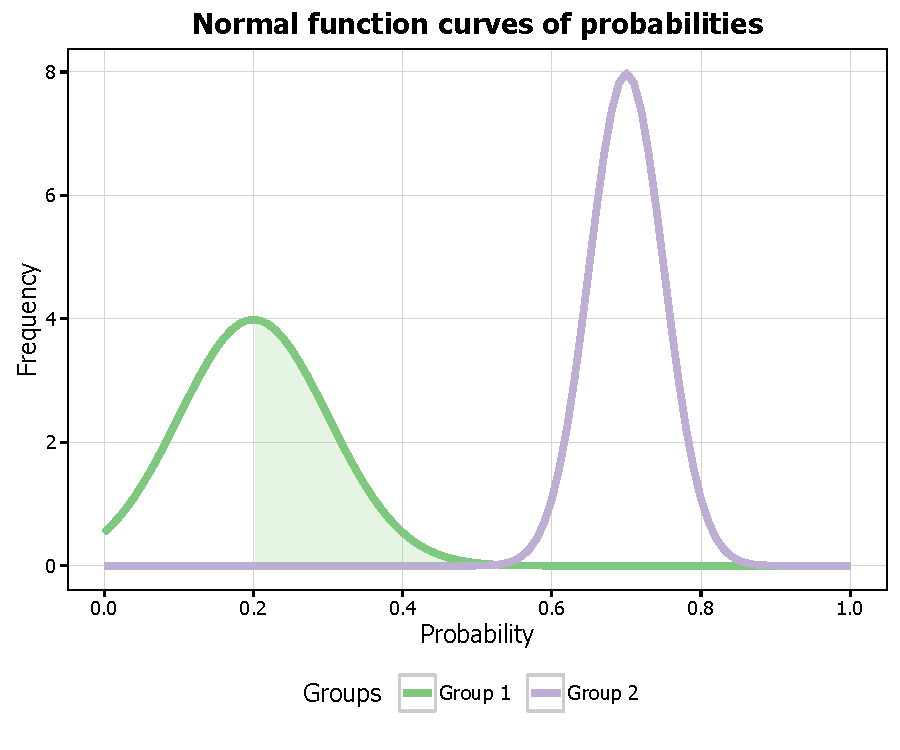
\includegraphics[width=0.6\linewidth]{9_Function_Plots_pdf/function_19-1} \end{center}
